\documentclass[11pt]{article}
\usepackage[utf8]{inputenc}
\usepackage[russian]{babel}
\usepackage[T1]{fontenc}
\usepackage{amssymb,amsmath,clrscode,graphicx,indentfirst}

\setlength{\parskip}{1ex plus 0.5ex minus 0.2ex}
\newcommand\doubleplus{+\kern-1.3ex+\kern0.8ex}

\author{Олег Смирнов\\
\texttt{oleg.smirnov@gmail.com}}
\date{8 декабря 2011 г.}
\title{Построение и анализ алгоритмов -- Лекция 10. Двоичные поисковые деревья}

\begin{document}

\maketitle
\tableofcontents
\newpage

\setlength{\parskip}{1ex plus 0.5ex minus 0.2ex}

\section*{Цель лекции}
\begin{itemize}
\item Двоичные поисковые деревья.
\item Обход дерева и варианты записи дерева.
\item Связь с Quicksort.
\end{itemize}

\section{Двоичные и $N$-арные деревья}
В теории графов, дерево -- это связный (ориентированный или неориентированный)
граф, не содержащий циклов. Т.е. для любой вершины есть один и только один способ
добраться до любой другой вершины.

В программировании наиболее часто используются бинарные деревья, в которых число
исходящих рёбер не превосходит 2, и $N$-арные деревья с произвольным количеством
исходящих ребер.

В памяти компьютера деревья обычно представляют в виде связной структуры, где
каждый узел помимо ключа ($key$) хранит указатели на дочерние узлы и иногда на
родительский. Для хранения $N$-арных деревьев используют структуру с левым
дочерним и правыми сестринским узлами (left-child, right-sibling representation).
В этом случае вместо указателя на дочерние узлы каждый узел $x$ хранит два
указателя:
\begin{itemize}
\item в $left\_child[x]$ -- указатель на крайний левый дочерний узел узла $x$;
\item в $right\_sibling[x]$ -- указатель на узел, расположенный на одном уровне
  с $x$ справа от него.
\end{itemize}

\subsection{Свойства деревьев}
\begin{enumerate}
\item Дерево не имеет кратных ребер и петель.
\item Любое дерево с $n$ узлами содержит $n-1$ ребро. Более того, конечный
  связный граф является деревом тогда и только тогда, когда $B-P = 1$,
  здесь $B$ -- число узлов, $P$ -- число рёбер графа.
\item Граф является деревом тогда и только тогда, когда любые два различных его
  узла можно соединить единственным элементарным путём.
\item Любое дерево однозначно определяется расстояниями (длиной наименьшей
  цепи) между его концевыми (степени 1) узлами.
\item Любое дерево является двудольным графом. Любое дерево, содержащее счётное
  количество вершин, является планарным графом.
\end{enumerate}

\section{Двоичные (бинарные) поисковые деревья}
Двоичным или бинарным поисковым деревом называется бинарное дерево, для
каждого узла $x$ которого выполняется следующее свойство:
\begin{itemize}
\item если узел $y$ лежит в левом поддереве узла $x$, то 
  $key[y] \leqslant key[x]$;
\item если узел $y$ лежит в правом поддереве узла $x$, то
  $key[y] \geqslant key[x]$.
\end{itemize}

``Хорошими'' считаются сбалансированные бинарные деревья с высотой
порядка $O(\lg n)$. У несбалансированных бинарных деревьев высота может
достигать $n$. Время прохода по бинарному дереву пропорционально его высоте.
Цель -- построить бинарное дерево с высотой порядка $O(\lg n)$ в большинстве
случаев. Один из способов -- рандомизация -- рассматривается в данной лекции.

\subsection{Сортировка массива}
Бинарные деревья поиска можно использовать для сортировки массива:
\begin{codebox}
\li $T \gets \emptyset $
\li \For $i \gets 1$ \To $n$
\li \Do Tree\_Insert($T$, $A[i]$)
  \End
\li Inorder\_Tree\_Walk(root$[T]$)
\end{codebox}

\begin{figure}[ht]
  \centering
  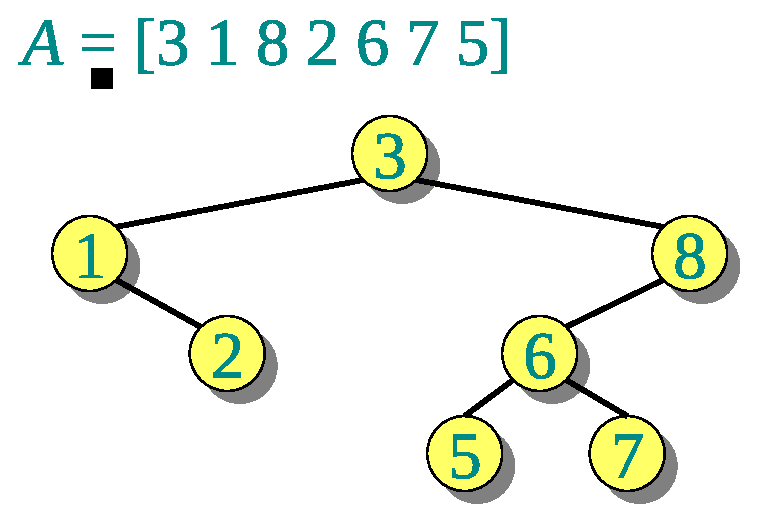
\includegraphics[width=2in]{lecture10/bs_tree.eps}
  \caption{Дерево работы BST sort}
  \label{fig:bs_tree}
\end{figure}

Время работы алгоритма складывается из частей:
\begin{itemize}
\item $O(n)$ для обхода Inorder\_Tree\_Walk.
\item $\Omega(n \lg n)$ для Tree\_Insert в среднем и в лучшем случае (идеально
  сбалансированное бинарное дерево).
\item $T = \sum_{x \in T} depth(x) = \Theta(n^2)$ для Tree\_Insert в худшем
  случае (массиво уже отсортирован).
\end{itemize}

Поведение алгоритма похоже на поведение сортирвки Хоара -- Quicksort.

\section{Бинарное поисковое дерево и сортировка Хоара}
Алгоритмы BST sort и Quicksort выполняют одинаковое количество сравнений, но в
различном порядке.
\begin{figure}[ht]
  \centering
  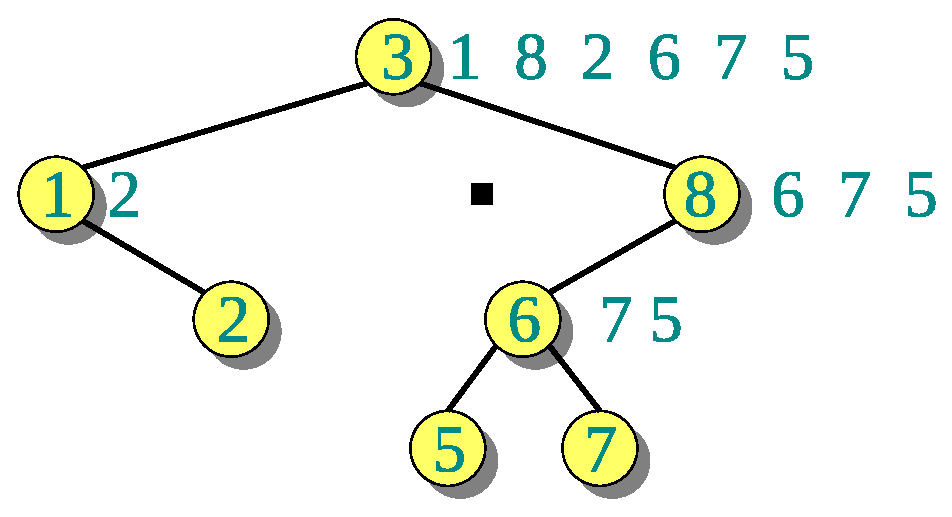
\includegraphics[width=2in]{lecture10/qs_tree.eps}
  \caption{Дерево работы Quicksort}
  \label{fig:qs_tree}
\end{figure}

Полученное дерево в точности совпадает с построенным в предыдущем примере.

Анализируя работу, можно увидеть, что алгоритм Quicksort в начале делает
сравнение всех элементов с первым опорным (3), генерируя первое разбиение.
BST sort также сравнивает каждый элемент в порядке добавления с корнем дерева
(3). Аналогичные сравнения происходят для каждого элемента массива.
Элемент, который в Quicksort становится опорным, в BST sort становится корнем
поддерева.

\subsection{Рандомизированный BST sort}
\begin{enumerate}
\item Случайная перестановка элементов массива
\item Сортировка BST sort(A)
\end{enumerate}

Время работы совпадает со временем рандомизированного Quicksort. Совпадает и
мат. ожидание:
\begin{equation*}
  E[\text{time}] = E[\text{Randomized\_Quicksort}] = \Theta(n \lg n)
\end{equation*}

Нет смысла использовать BST sort для сортировки массива, т.к. время не
отличается от Quicksort. Поиск по BST также не дает преимуществ по сравнению с
бинарным поиском в просто отсортированном массиве. Полезность BST заключается
в возможности добавлять элементы в структуру динамически, сохраняя ожидаемое
время работы.

Ожидаемое время работы рандомизированного алгоритма BST sort $T(n)$ будет
$\Theta(n \lg n)$. Время работы равно сумме глубины всех узлов дерева:
\begin{equation*}
  T(n) = \sum_{x} depth~x
\end{equation*}

\section{Анализ высоты BST}
Интуитивно ясно, что ожидаемая высота дерева должна быть $\Theta(\lg n)$.

Ожидаемая \emph{средняя} высота будет равна: $E[\frac{1}{n}\sum_{x \in T}
depth~x] = \frac{\Theta(n \lg n)}{n} = \Theta(\lg n)$.

Ожидаемая средняя высота дерева $\Theta(\lg n)$ не означает, что высота всего
дерева также будет $\Theta(\lg n)$. Например, если в дереве есть один из путей
длинной $\sqrt(n) > \lg n$, а остальные пути $\lg{n - \sqrt(n)}$, средняя
высота, тем не менее, будет равна:
\begin{equation*}
 \leqslant \frac{1}{n}(n \lg n + \sqrt(n) \sqrt(n)) = O(\lg n)
\end{equation*}

Теорема: $E[\text{высота рандомизированного BST}] = O(\lg n)$

Доказательство теоремы позволит показать, что в рандомизированном BST можно
производить поиск за (ожидаемое) логарифмическое время.

Схема доказательства:
\begin{enumerate}
\item Неравенство Йенсена для выпуклой функции $f$: $f(E[X]) \leqslant E[f(X)]$.
\item Вместо анализа $X_n$ (случайная величина высоты BST) анализ
  $Y_n = 2^{X_n}$.
\item Доказательство $E[Y_n] = O(n^3)$.
\item Поиск границы $E[2^{X_n}] = E[Y_n] = O(n^3)$.
\item В соответствии с неравенством Йенсена $2^{E[X_n]} \leqslant E[2^{X_n}]$.
\item После логарифмирования получим $E[X_n] \leqslant \lg O(n^3) = 3\lg n +
  O(1)$.
\end{enumerate}

\subsection{Ожидаемая высота}
Пусть $X_n$ -- случайная величина высоты рандомизированного BST для $n$ узлов,
а $Y_n = 2^{X_n}$ -- выпуклая функция.

Анализ высоты дерева похож на анализ алгоритма Quicksort в том смысле, что после
выбора корня дерева $r$ остальные элементы исходного массива разделяются на две
части -- меньшие $r$ (пусть $k$ элементов), которые попадут в левое поддерево и
большие $r$ ($n - k - 1$), которые попадут в правое поддерево. Каждое из
поддеревьев также является случайным рандомизированным BST, что приводит к
рекурсивному анализу алгоритма.

Если корень дерева $r$ имеет ранг $k$, то $X_n = 1 + \max(X_{k-1}, X{n-k})$,
а $Y_n = 2max(Y_{k-1}, Y_{n-k})$.

Можно показать, что 
\begin{equation*}
  E[X_n] \leqslant 3 \lg n + O(1) \\  
\end{equation*}

\section{Алгоритмы работы с бинарными деревьями}
Пусть высота бинарного дерева равна $h$. Тогда алгоритм поиска элемента
$k$ в дереве с корнем $x$ выполняется за время $O(h)$:
\begin{codebox}
\Procname{$\proc{Tree\_Search}(x, k)$}
\li \If $x = NIL$ | $k = key[x]$
\li \Then \Return $x$
\End
\li \If $k < key[x]$
\li \Then \Return $Tree\_Search(left[x], k)$
\li \Else \Return $Tree\_Search(right[x], k)$
\End
\end{codebox}
Процедуру можно превратить в итеративную с помощью хвостовой рекурсии.

\subsection{Обход дерева}
Поиск элемента в дереве является частным случаем процедуры обхода дерева.
Существует несколько принципиально разных способов обхода:
\begin{enumerate}
\item Обход в прямом порядке, когда каждый узел посещается до того, как
  посещены его потомки ($prefix$ $traverse$). Для корня дерева рекурсивно
  вызывается следующая процедура:
  \begin{enumerate}
  \item Посетить узел.
  \item Обойти левое поддерево.
  \item Обойти правое поддерево.
  \end{enumerate}
  Такой обход используется, например, в решение задачи методом деления на части
  и в стратегии ``разделяй и властвуй'' (сортировка слиянием, быстрая 
  сортировка, одновременное нахождение максимума и минимума последовательности
  чисел, умножение длинных чисел и т.д.).
\item Симметричный обход, когда сначала посещается левое поддерево, затем
  узел, затем правое поддерево ($infix$ $traverse$). Для корня дерева рекурсивно
  вызывается следующая процедура:
  \begin{enumerate}
  \item Обойти левое поддерево.
  \item Посетить узел.
  \item Обойти правое поддерево.
  \end{enumerate}
\item Обход в обратном порядке ($postfix$ $traverse$), когда узлы посещаются
  ``снизу вверх'' по следующей процедуре:
  \begin{enumerate}
  \item Обойти левое поддерево.
  \item Обойти правое поддерево.
  \item Посетить узел.
  \end{enumerate}
  Такой обход используется в анализе игр с полной информацией и в динамическом
  программирование.
\item Обход в ширину, когда узлы посещаются уровень за уровнем ($N$-й уровень
  дерева -- множество узлов с высотой $N$). Каждый уровень обходится слева
  направо. Для его реализации используется структура $queue$ (очередь).
\end{enumerate}

\subsection{Вставка и удаление элемента}
Алгоритм вставки узла $z$, у которого $key[z] = v$, $left[z] = NIL$,
$right[z] = NIL$ в дерево $T$:
\begin{codebox}
\Procname{$\proc{Tree\_Insert}(T, z)$}
\li $y \gets NIL$
\li $x \gets root[T]$
\li \While $x \neq NIL$
\li   \Do $y \gets x$
\li     \If $key[z] < key[x]$
\li       \Then $x \gets left[x]$
\li       \Else $x \gets right[x]$
  \End
\End
\li $p[z] \gets y$
\li \If $y = NIL$
\li   \Then $root[T] \gets z$ \Comment Дерево T -- пустое
\li   \Else \If $key[z] < key[y]$
\li       \Then $left[y] \gets z$
\li       \Else $right[y] \gets z$
  \End
\End
\end{codebox}

Цикл в начале процедуры перемещает указатели вниз по дереву в зависимости от
сравнения ключей $key[x]$ и $key[z]$, до тех пор, пока $x$ не станет равным NIL.
Это значение находится именно в той позиции, куда следует вставить узел $z$.

Процедура Tree\_Delete рассматривает три возможных случая:
\begin{enumerate}
\item Если у узла $z$ нет дочерних узлов, он просто удаляется из дерева;
\item Если у узла один дочерний узел, он ``склеивается'' с родительским для $z$;
\item Если дочерних узла два, то в дереве находим следующий за $z$ узел $y$, у
  которого нет левого дочернего узла, убираем его из позиции, где он находился
  ранее и заменяем им узел $z$.
\end{enumerate}

Можно показать, что если у узла BST два дочерних узла, то у предшествующего
узла нет правого дочернего, а у последующего -- левого.

Если в дереве $T$ существуют два узла $a$ и $b$, $a < b$, такие, что
$rank(a) = k$, $rank(b) = k+1$. Т.е. узел $b$ является последующим за $a$.
Левым дочерним узлом узла $b$ может являтся только элемент $x < b$. Но из
условия предшествия следует, что $x < a$ и $rank(x) < rank(a)$. Т.к. узлы
$a$ и $b$ уже размещены в дереве, алгоритм Tree\_Insert поместит $x$ в
левое поддерево элемента $a$, но не $b$.

Процедура Tree\_Successor возвращает следующий элемент за аргументом в
отсортированной последовательности.

\begin{codebox}
\Procname{$\proc{Tree\_Delete}(T, z)$}
\li \If $left[z] = NIL$ | $right[z] = NIL$
\li   \Then $y \gets z$
\li   \Else $y \gets Tree\_Successor(z)$
  \End
\li \If $left[y] \neq NIL$
\li   \Then $x \gets left[y]$
\li   \Else $x \gets right[y]$
  \End
\li \If $x \neq NIL$
\li   \Then $p[x] \gets p[y]$
  \End
\li \If $p[y] = NIL$
\li   \Then $root[T] \gets x$
\li   \Else \If $y = left[p[y]]$
\li         \Then $left[p[y]] \gets x$
\li         \Else $right[p[y]] \gets x$
  \End
\End
\li \If $y \neq z$
\li   \Then $key[z] \gets key[y]$
\li   \Comment Копирование сопутствующих данных в $z$
  \End
\li \Return $y$
\End
\end{codebox}

Очевидно, что балансировку дерева можно нарушить, вставляя или удаляя специально
подобранные элементы. Для борьбы с таким поведением существуют специальные
структуры данных и соответствующие алгоритмы: красно-чёрные деревья, AVL-деревья,
декарторвы деревья (Treap) и т.п.
\end{document}
